%%=============================================================================
%% Methodologie
%%=============================================================================

\chapter{\IfLanguageName{dutch}{Methodologie}{Methodology}}%
\label{ch:methodologie}

Dit hoofdstuk biedt een gestructureerd overzicht van de methodologische aanpak die is gehanteerd in dit onderzoek. Het is bedoeld om de lezer inzicht te geven in de onderzoeksopzet, de gehanteerde methoden en de rationale achter de gekozen aanpak. Het onderzoek is opgedeeld in verschillende fasen, elk met specifieke doelstellingen, deliverables, en onderzoeksmethoden. De onderstaande secties beschrijven deze fasen in detail.

%Literatuurstudie
De eerste fase van het onderzoek bestond uit een uitgebreide literatuurstudie, gericht op het verkennen van het bestaande kennisdomein met betrekking tot 'secondary babytalk', de beschikbare spraak-naar-tekst \gls{asr} modellen, en de criteria voor model evaluatie. Deze fase had als doelstelling het vaststellen van een theoretische basis voor het onderzoek.

%Selectie van ASR Modellen

In de literatuurstudie kwam een fase waarbij bepaalde \gls{asr} modellen uitgekozen werden voor een analyse. De keuze voor deze modellen was gebaseerd op de beschikbaarheid en ondersteuning van het Vlaamse en Nederlandse taal. Die modellen zullen dan gebruikt worden om de steekproefneming te transcriberen.



De volgende stap in het proces is het verzamelen van audio samples. Deze samples zullen vervolgens worden onderworpen aan de geselecteerde AI-modellen voor transcribering. Het doel is om elke sample te laten transcriberen door de AI-modellen. 
De resulterende transcribties, samen met de grondwaarheid 'Ground truth' transcribties, worden vervolgens gebruikt als parameters voor de Jiwer-bibliotheek om de relevante metrics te berekenen. Een diagram in figuur \ref{fig:plan_methodologie} toont de wijze waarop de evaluatieprocedure zal worden uitgevoerd.
\\

Na het verzamelen van de resultaten van deze evaluatie, worden ze samengebracht en overzichtelijk gepresenteerd in een tabel. Deze tabel zal een gedetailleerd inzicht bieden in de prestaties van de AI-modellen op basis van verschillende metrics en criteria. 

\begin{figure}[h]
    \centering
    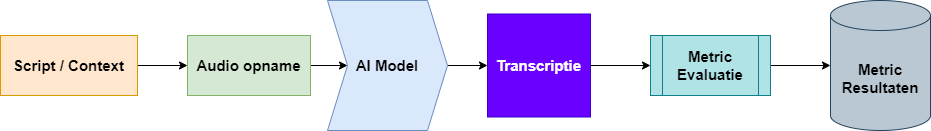
\includegraphics[width=0.8\textwidth]{plan.png}
    \captionsetup{justification=centering}
    \caption{Het uitvoeringsplan voor de evaluatieprocedure.}
    \label{fig:plan_methodologie}
\end{figure}


Ten slotte zal er op basis van de analyse van de resultaten een beslissing worden genomen. Deze beslissing kan betrekking hebben op verdere optimalisatie van de AI-modellen, het identificeren van zwakke punten in het systeem, of het bepalen van de geschiktheid van de AI-modellen voor het beoogde gebruiksscenario.

